%!TeX root = ../principal.tex
%!TeX encoding = utf-8
\chapter{Classe FEECTeX}
\label{cap1}

\section{Citações}

Considerando que as referências estejam armazenadas no arquivo \textit{bibliografia.bib} na pasta raíz, as citações podem ser feitas através dos comandos:

\begin{itemize}
    \item \verb|\citar{<chave#1>, <chave#2>, ..., <chave#n>}|;
    \item \verb|\citarautora{<chave>}| ou \verb|\citarautor{<chave>}|;
    \item \verb|\citarano{<chave>}|.
\end{itemize}

\noindent Exemplos: \verb|\citar{autor, autora}| produz \citar{autor, autora}. \verb|\citar| \verb|autora{autora}| produz \citarautora{autora}; \verb|\citarano{autora/autor}| produz \citarano{autora}.

\section{Notas de Rodapé}

As notas de rodapé são declaradas através do comando \verb|\footnote{<nota>}|, por exemplo: a classe \feectex é derivada da classe abntex2\footnote{O abnTeX2 é uma evolução do abnTeX -- ABsurd Norms for TeX.}.

\section{Abreviaturas e siglas}

A lista de abreviaturas e siglas é gerada automaticamente. Para que isso aconteça, basta que os comandos \verb|\abreviatura{<abreviatura>}| \verb|{<definição>}|, \verb|\sigla| \verb|{<sigla>}{<definição>}| sejam encontrados durante a preparação do documento PDF.

Exemplos: \verb|\sigla{ABNT}{Associação Brasileira de Normas Técnicas}| e \verb|\abreviatura{Dr.}{Doutor}| produzem a sigla e a abreviatura listadas na lista de abreviaturas e símbolos.\sigla{ABNT}{Associação Brasileira de Normas Técnicas} \abreviatura{Dr.}{Doutor}

\section{Símbolos}

Assim como lista de abreviaturas e siglas, a lista de símbolos também é gerada automaticamente. Da mesma maneira, basta que o comando \verb|\simbolo<símbolo>}| \verb|{<definição>}| seja encontrado ao longo da preparação do documento PDF para que isso aconteça.

Exemplo: \verb|\simbolo{$\mathbb{R}$}{Conjunto dos números reais}| produz o símbolo listado na lista de símbolos. \simbolo{$\mathbb{R}$}{Conjunto dos números reais}

\section{Tabelas}

\begin{table}
    \centering
    \begin{tabular}{c | c}
        \hline
        Autor & Obra \\
        \hline
        Akira Toriyama & Dragon Ball \\
        Carlos Drummond de Andrade & De Notícias \& Não Notícias Faz-Se a Crônica
    \end{tabular}
    \caption[Tabela]{Tabela de autores e obras.}
    \label{table:1}
\end{table}

\section{Figuras}

O tamanho das imagens pode ser escolhido através dos comandos \verb|width| e \verb|scale|.

\begin{figure}[h!]
    \centering
    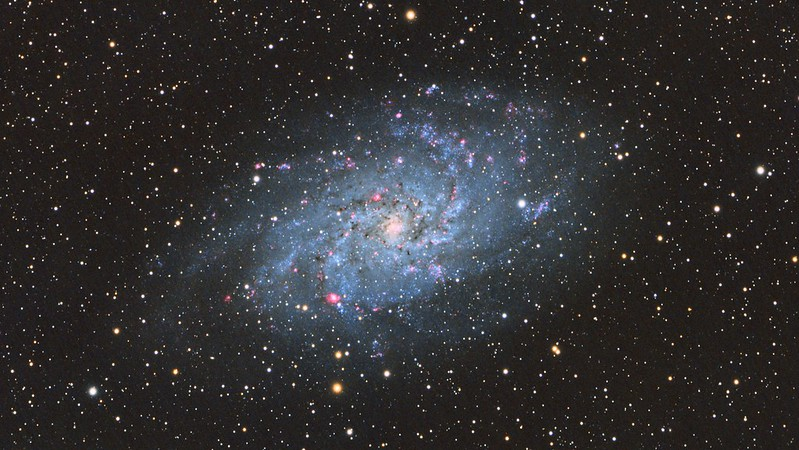
\includegraphics[width=0.8\textwidth]{capitulo-1/28421613139_a4472645e5_c.jpg}
    \caption[Galáxia M33]{Galáxia do Triângulo M33.}
\end{figure}

% \begin{figure}
%     \centering
%     \begin{subfigure}[b]{0.3\textwidth}
%         \centering
%         \includegraphics[width=\textwidth]{graph1}
%         \caption{$y=x$}
%         \label{fig:y equals x}
%     \end{subfigure}
%     \hfill
%     \begin{subfigure}[b]{0.3\textwidth}
%         \centering
%         \includegraphics[width=\textwidth]{graph2}
%         \caption{$y=3\sin x$}
%         \label{fig:three sin x}
%     \end{subfigure}
%     \hfill
%     \begin{subfigure}[b]{0.3\textwidth}
%         \centering
%         \includegraphics[width=\textwidth]{graph3}
%         \caption{$y=5/x$}
%         \label{fig:five over x}
%     \end{subfigure}
%        \caption{Three simple graphs}
%        \label{fig:three graphs}
% \end{figure}
